\section{Equality and the family of extremizers}\label{sec:5}

\subsection{The complete equality condition}\label{sec:5.1}

Continue in John coordinates and write
\begin{equation}\label{eq:5.1}
\mathcal Z_b=\{-v\}\cup\{u\in S^{n-1}:u^Tv=b\}.
\end{equation}

This set consists of the pole opposite the cut direction and a latitude sphere. The extremal ellipsoid $\mathcal E(c_*,A_*)$ is the one defined in \eqref{eq:3.2}.

\begin{theorem}[{equality classification}]\label{thm-equality}
A normalized body $K$ attains $w(K\cap H_v)=R_nw(K)$ if and only if it admits a John frame supported on $\mathcal Z_b$ such that
\begin{equation}\label{eq:5.2}
\operatorname{conv}\bigl(B_2^n\cup\mathcal E(c_*,A_*)\bigr)
\subseteq K\subseteq P_{\mathcal U}.
\end{equation}

The new John ellipsoid is then exactly $\mathcal E(c_*,A_*)$. If equality holds, every positive-weight John frame supporting $K$ lies in $\mathcal Z_b$. For a contact polytope $P_{\mathcal U}$, equality is equivalent simply to its defining John frame being supported on $\mathcal Z_b$.

\end{theorem}

\begin{proof}
For necessity, zero deficit will first determine the contact heights
and ellipsoid shape, then the active supports will determine its center.
For sufficiency, the candidate ellipsoid in the sandwich already supplies the
required volume.

\textbf{Necessity: recover the shape and then the center.} Fix any supporting John
frame and suppose $\det A=R_n$. The deficit identity gives
\begin{equation}\label{eq:5.3}
\begin{aligned}
\epsilon=0&\ \Longrightarrow\ \Delta_{\rm geom}=\mathcal C=\mathcal D=0\\
&\ \Longrightarrow\ \chi=0,\quad Q=M=M_0,\quad U=I,\quad A=A_*.
\end{aligned}
\end{equation}

The shape is now fixed. To recover the center, compare the active support
values with those of the model. Since $\alpha_i>0$ and
$p_i=A_*u_i/\|A_*u_i\|$, complementarity reduces to
\begin{equation}\label{eq:5.4}
0=\gamma_i
=\alpha_i\bigl(1-u_i^Tc-\|A_*u_i\|\bigr),
\qquad
u_i^T(c-c_*)=0\quad\forall i.
\end{equation}

The second identity uses the model support equations. Isotropy now recovers the center:
\begin{equation}\label{eq:5.5}
\|c-c_*\|^2
=\sum_i\lambda_i\bigl(u_i^T(c-c_*)\bigr)^2=0.
\end{equation}

Thus $\mathcal E(c_*,A_*)\subseteq K\cap H_v$, and convexity yields the left inclusion in \eqref{eq:5.2}. The right inclusion is \eqref{eq:2.18}. The frame was arbitrary, proving the asserted quantifier over every John frame.

\textbf{Sufficiency: use the included model ellipsoid.} Suppose \eqref{eq:5.2} holds for a
John frame supported on $\mathcal Z_b$. John's characterization and the model
feasibility give
\begin{equation}\label{eq:5.6}
w(K)=\kappa_n,\qquad
w(K\cap H_v)\ge\kappa_n\det A_*=R_n\kappa_n.
\end{equation}

Theorem~\ref{thm-sharp} supplies the reverse inequality. For $K=P_{\mathcal U}$, model feasibility follows directly from the three support values in Section~\ref{sec:3.2}. 
\end{proof}

The equality condition determines the new ellipsoid and the active contact geometry. It leaves freedom in the rest of the body, as the two inclusions in \eqref{eq:5.2} show.

\subsection{Extremizers beyond regular simplices}\label{sec:5.2}

The latitude part of an equality frame can be built from any John frame in one lower dimension. This gives a concrete description of the freedom in Theorem~\ref{thm-equality}.

\begin{proposition}[{transverse construction}]\label{prop-extremizers}
Let unit vectors $w_i\in v^\perp$ and positive weights $\mu_i$ satisfy
$\sum_i\mu_iw_i=0$ and $\sum_i\mu_iw_iw_i^T=P$. Then the contacts
\begin{equation}\label{eq:5.7}
u_i=bv+\sqrt{1-b^2}\,w_i,\qquad
\lambda_i=\frac{\mu_i}{1-b^2},\qquad
u_{\rm pole}=-v,\qquad \lambda_{\rm pole}=\frac1{1+b}
\end{equation}
form a John frame supported on $\mathcal Z_b$.

\end{proposition}

\begin{proof}
The weight rescaling compensates for the transverse length
$\sqrt{1-b^2}$, while the pole weight balances the axial first moment.
We check that the same choices also give the axial second moment.
The vectors have unit norm because $w_i\perp v$ and
$\|u_i\|^2=b^2+(1-b^2)\|w_i\|^2=1$. Taking traces in the transverse second moment gives
\begin{equation}\label{eq:5.8}
\sum_i\mu_i=n-1=\frac{1-b}{b},\qquad
S:=\sum_i\lambda_i=\frac1{b(1+b)}.
\end{equation}

The pole and latitude contributions therefore satisfy
\begin{equation}\label{eq:5.9}
\begin{aligned}
\lambda_{\rm pole}u_{\rm pole}+\sum_i\lambda_i u_i
&=\left(-\frac1{1+b}+bS\right)v
+\frac1{\sqrt{1-b^2}}\sum_i\mu_iw_i=0,\\
\lambda_{\rm pole}u_{\rm pole}u_{\rm pole}^T+\sum_i\lambda_i u_i u_i^T
&=\left(\frac1{1+b}+b^2S\right)vv^T+\sum_i\mu_iw_iw_i^T\\
&=vv^T+P=I.
\end{aligned}
\end{equation}

The mixed terms in the second line vanish by $\sum_i\mu_iw_i=0$. All weights are positive and all heights lie in $\{-1,b\}$. 
\end{proof}

For example, take $w_i=\pm e_j$, $j=1,\ldots,n-1$, with $\mu_i=1/2$. In dimension three, set $v=e_3$. The four latitude contacts have John weight $9/16$ each, and the pole $-e_3$ has weight $3/4$. Their contact polytope is the square pyramid
\begin{equation}\label{eq:5.10}
K=\{(x,y,z):z\ge-1,\quad
2\sqrt2|x|+z\le3,\quad 2\sqrt2|y|+z\le3\}.
\end{equation}

Its base vertices are $(\pm\sqrt2,\pm\sqrt2,-1)$ and its apex is $(0,0,3)$. Proposition~\ref{prop-extremizers} and Theorem~\ref{thm-equality} give $J(K)=B_2^3$ and
\begin{equation}\label{eq:5.11}
\begin{gathered}
J(K\cap\{z\le0\})=c_*+A_*B_2^3,\qquad
c_*=-\frac12e_3,\\
A_*=\operatorname{diag}\!\left(\sqrt{\frac32},\sqrt{\frac32},\frac12\right),
\qquad \frac{w(K\cap\{z\le0\})}{w(K)}=\det A_*=\frac34=R_3.
\end{gathered}
\end{equation}

\begin{figure}[tbp]
\centering
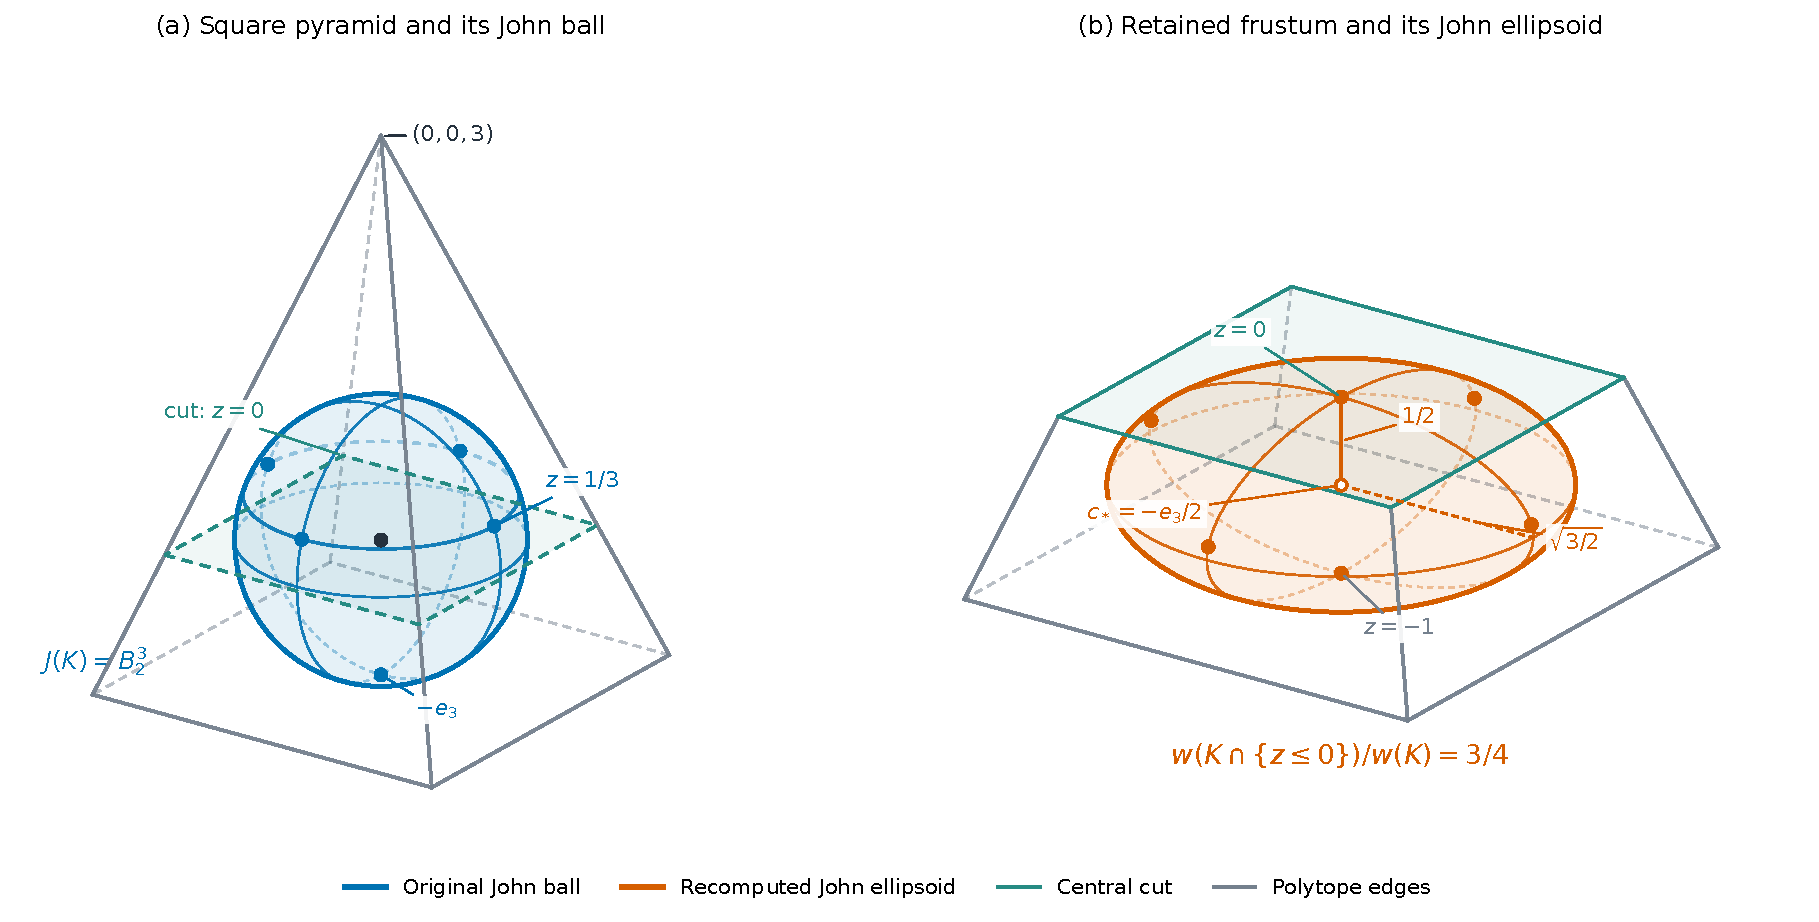
\includegraphics[width=0.98\linewidth]{figures/square_pyramid.pdf}
\caption{A square-pyramid extremizer in dimension three. (a) The unit ball touches four triangular side facets at height $z=1/3$ and the square base at $-e_3$. (b) The central cut leaves a square frustum. Its John ellipsoid touches the four sides, the base, and the cut; its semiaxes are $\sqrt{3/2},\sqrt{3/2},1/2$. Filled colored points mark contacts, and the open orange point marks the new center. Both panels use the same orthographic viewing direction, with an enlarged view in (b). This five-facet extremizer exhibits the freedom beyond the simplex model in Figure~\ref{fig:1}.}\label{fig:2}
\end{figure}

The regular tetrahedron is therefore only one member of the three-dimensional equality family. Any body between the two sets in \eqref{eq:5.2} is also an extremizer.

This has a direct consequence for stability. Near equality should force proximity to the common extremal ellipsoid and contact family. It cannot force every body to be close to a unique simplex.
